\section{Visualization Examples}
\label{sec:examples}

In this section, some examples of visualization from the literature will be discussed. The visualizations are grouped by their intended use case for the dashboard.

\subsection{Success Prediction}
\label{subsec:success_prediction}

The first group of visualizations is concerned with predicting student success.

One quite intuitive design element here is a traffic light scheme, with green indicating a high likelihood of success, yellow indicating a moderate likelihood, and red indicating a low likelihood. This can be seen in the success score gauge plot in Figure \ref{fig:trajectory}.

In this plot, there are multiple zones, indicating different risk levels. This plot focuses on derived data and can be used to highlight the likelihood of failure for a given course or the degree program as a whole. Additionally, a second indicator can be added to this plot, to highlight the effect of an intervention or a change in study behavior.


\begin{figure}
    \centering
    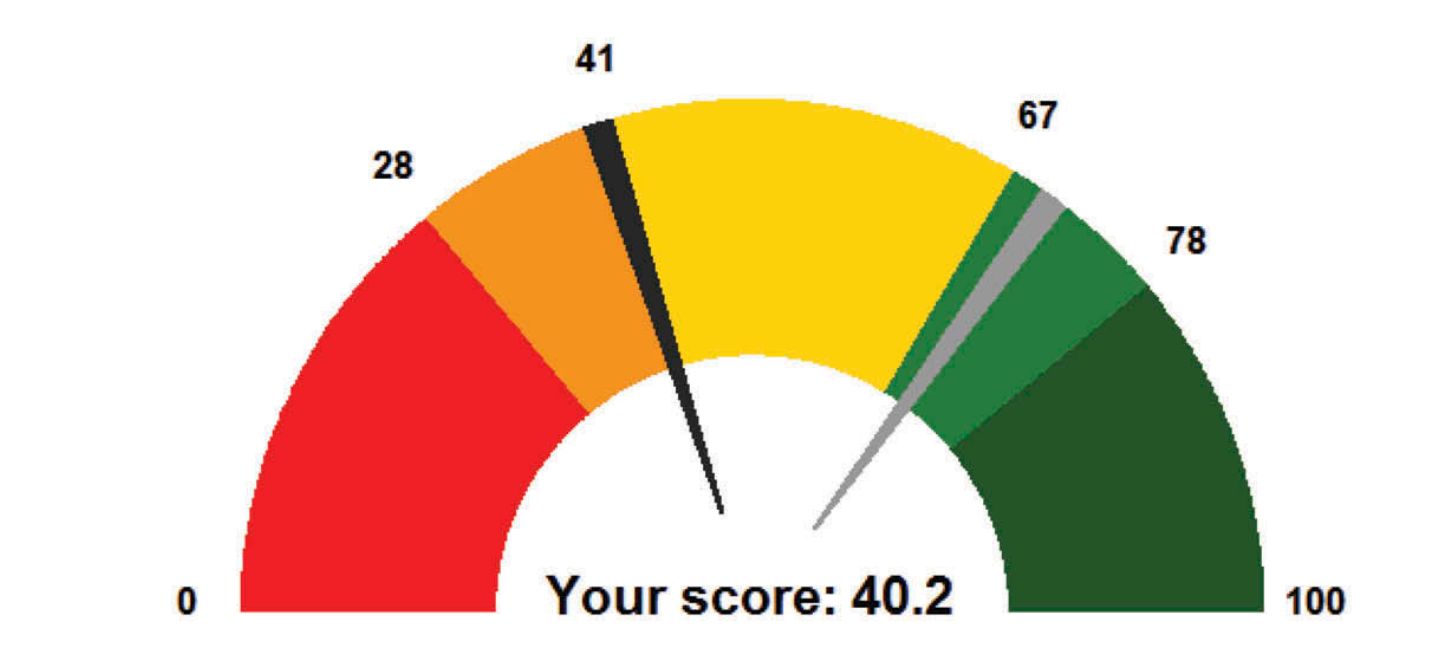
\includegraphics[width=0.8\textwidth]{figures/success_1.png}
    \caption{Success score gauge plot, from \cite{PredictingSuccess}}
    \label{fig:trajectory}
\end{figure}

Success prediction can also be helpful when planning which exams to take. In Figure \ref{fig:succes_2.png}, a student can select which exams they intend to take, and the system will predict the likelihood of passing all selected exams.
This can help students to focus on fewer exams instead of taking all exams at once.

\begin{figure}
    \centering
    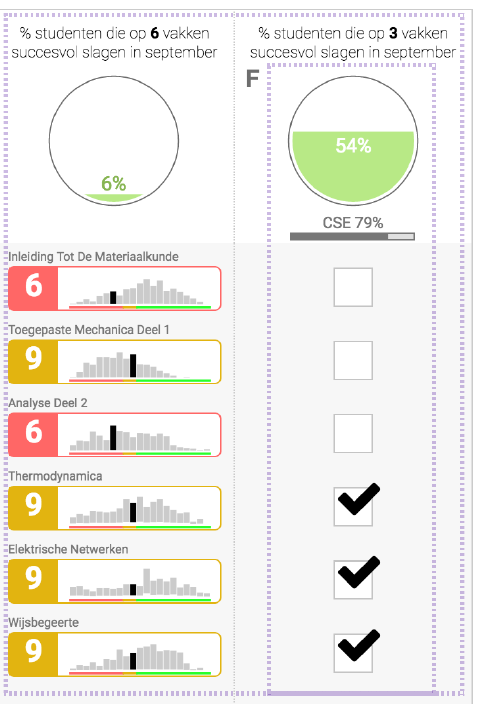
\includegraphics[width=0.4\textwidth]{figures/success_2.png}
    \caption{Success prediction for selected exams, from \cite{LISSA}}
    \label{fig:succes_2.png}
\end{figure}

\subsection{Trajectory}
\label{subsec:trajectory}

Another group of visualizations is concerned with the trajectory of a student.
These can be used to show the path, a student has taken so far and is likely to take in the future. This can be helpful to identify students who are at risk of dropping out or to suggest interventions to students who are likely to take longer than expected to finish their degree.

In Figure \ref{fig:trajectory_1.png}, a selection of typical trajectories is shown.
These have been identified by the Authors of \cite{DegreePictures-Seed} and experienced educators.
The trajectories might be used to identify students at risk of dropping out, by comparing their actual grade history to the typical trajectories. There remains the risk, however, that the pattern might become apparent only after the optimal intervention time has passed already.

Figure \ref{fig:trajectory_2.png} shows multiple trajectories for the same student.
The top left plot shows the trajectory over all courses, while the other panels plot achievements for different categories of courses.
This can be used to get more nuanced insights into the performance of a student, who might be doing well in some categories, but poorly in others.
The insights could be used to inform decisions about which actions to take: for example, non-mandatory courses could be selected from the areas in which the student performs better, the student could invest more time into the courses in which they perform worse or a possible intervention could target the categories where the student is struggling.

\begin{figure}
    \begin{minipage}[b]{0.48\textwidth}
        \centering
        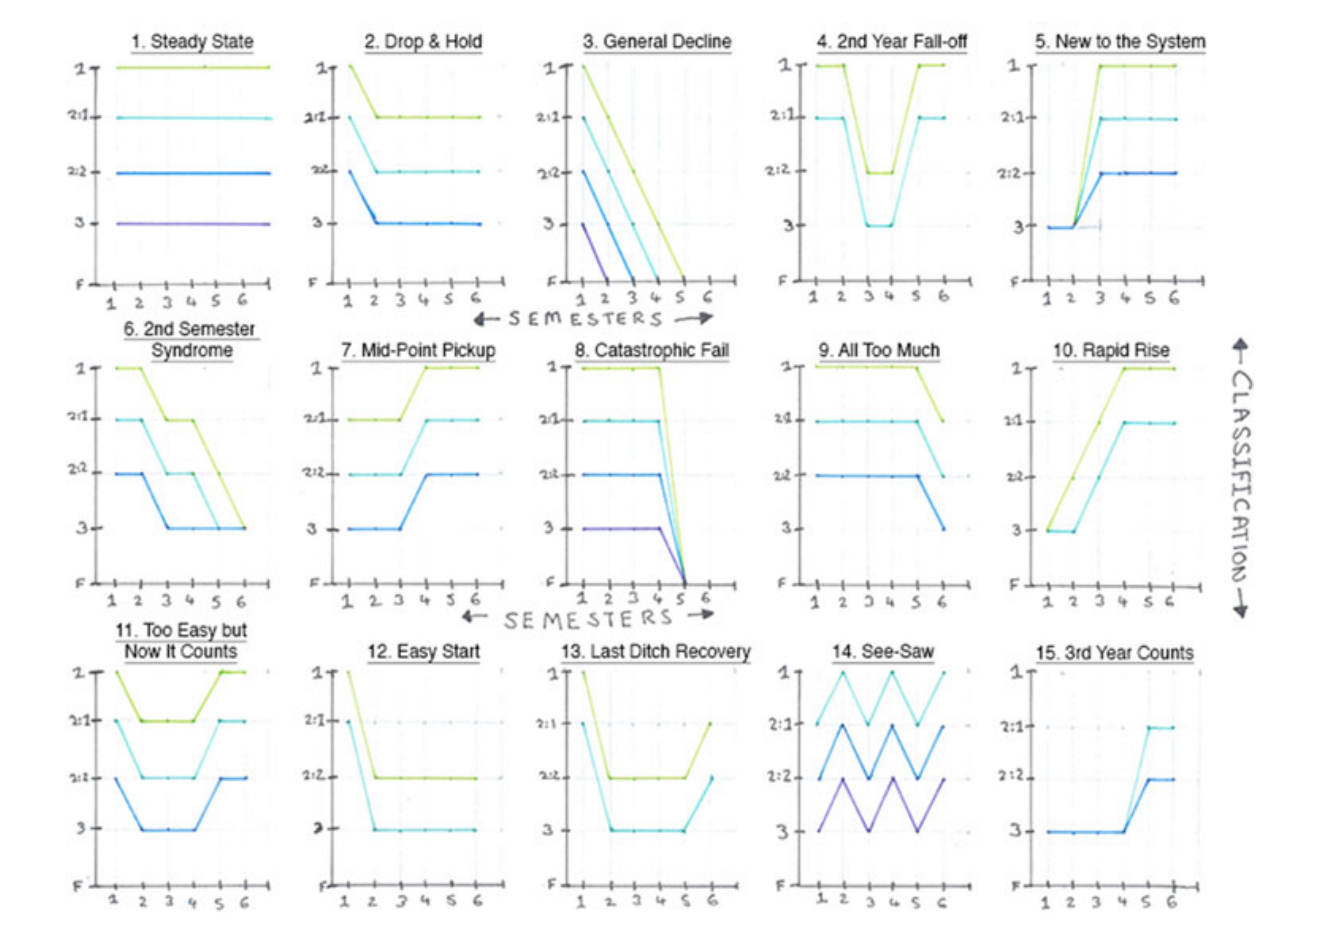
\includegraphics[width=0.8\textwidth]{figures/trajectory_1.png}
        \caption{Selection of typical trajectories, from \cite{DegreePictures-Seed}}
        \label{fig:trajectory_1.png}
    \end{minipage}
    \hfill
    \begin{minipage}[b]{0.48\textwidth}
        \centering
        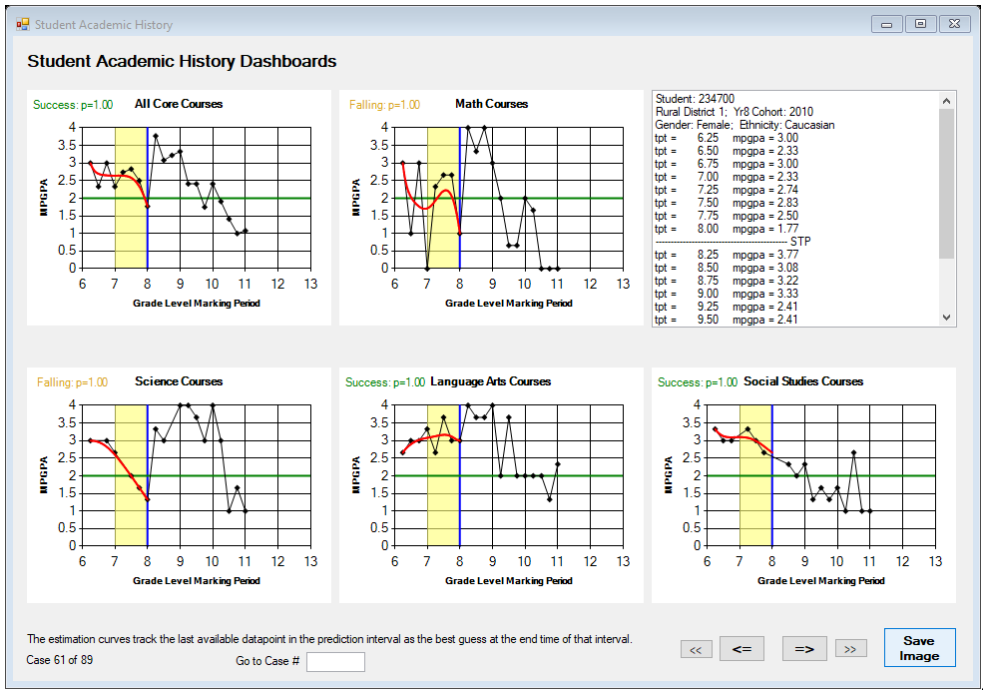
\includegraphics[width=0.8\textwidth]{figures/trajectory_2.png}
        \caption{Trajectory of a student for different course bundles, from \cite{Longitudinal-StudentPerformance}}
        \label{fig:trajectory_2.png}
    \end{minipage}
\end{figure}

In Figure \ref{fig:trajectory-finish_1.png}, estimates for the completion of the study program are shown. Compared to students with a similar profile, this shows the proportion of students that finished their degree program in three, four or five years and the proportion of students that dropped out. This can be useful in the planning phases, as the differences can be compared when selecting different courses for example. Additionally, the influence of passing or failing a given exam can be visualized in such a way.



\subsection{Comparison with cohorts}
\label{subsec:comparison}

The Comparison with other students is a particularly interesting area. However, as will be discussed in Section \ref{sec:challenges}, some things need to be considered when comparing students with each other.

There are multiple dimensions, in which a comparison to other students could be helpful. The first one is the exam-level comparison, where the performance of a given student is compared to other students who took the same exam. This can also give an indication of the difficulty of the exam. Figure \ref{fig:comparison_exam.png} shows a histogram of grades for a given exam. Additionally, grades that constitute a pass or a fail are highlighted and the grade actually achieved by the student is shown. Figure \ref{fig:comparison_course.png} displays similar data differently: the distribution of final grades for a course is displayed as a donut chart.

\begin{figure}
    \begin{minipage}[b]{0.4\textwidth}
        \centering
        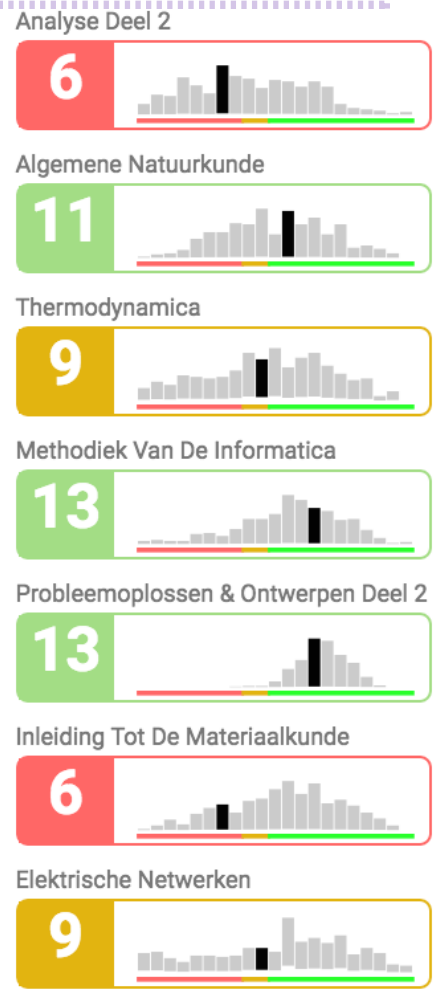
\includegraphics[width=0.9\textwidth]{figures/comp_exam.png}
        \caption{Distribution of grades for multiple exams, from \cite{LISSA}}
        \label{fig:comparison_exam.png}
    \end{minipage}
    \hfill
    \begin{minipage}[b]{0.4\textwidth}
        \centering
        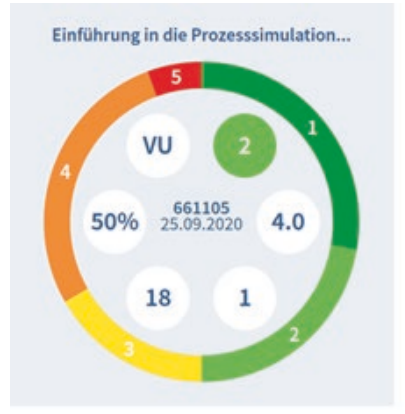
\includegraphics[width=0.9\textwidth]{figures/comp_course.png}
        \caption{Distribution of grades for a given course, from \cite{Dashboard-StudentProgress}}
        \label{fig:comparison_course.png}
    \end{minipage}


\end{figure}

Comparisons with other students can also play a role during the planning phase. Figure \ref{fig:comparison_ects.png} shows the amount of ECTS credits a given student is currently on track to achieve and the average amount of ECTS credits achieved by other students.
Additionally, thresholds are highlighted, that need to be cleared in order to meet certain requirements. This could also be adapted to the specific requirements of a given degree program.

\begin{figure}
    \centering
    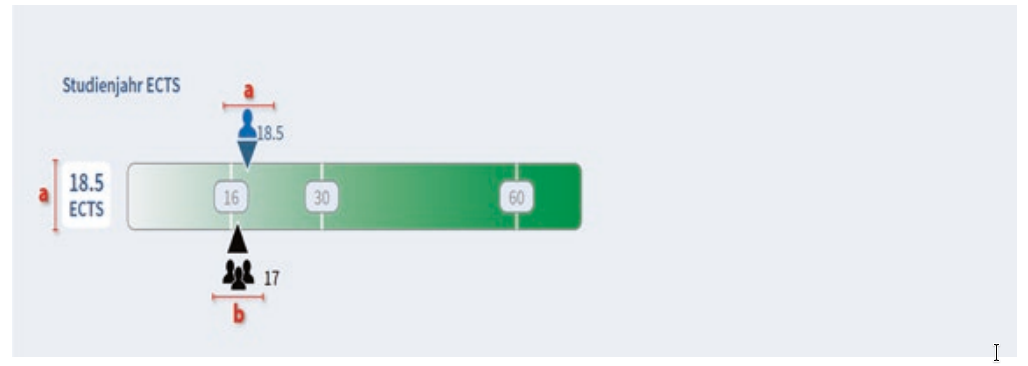
\includegraphics[width=0.5\textwidth]{figures/comp_ects.png}
    \caption{Comparison of ECTS credits achieved by a student and other students, from \cite{Dashboard-StudentProgress}}
    \label{fig:comparison_ects.png}
\end{figure}

Of course, some visualizations can belong to multiple groups. For example, Figure \ref{fig:comparison_trend} shows both the trajectory of a student and the performance compared to other students. The trajectory is shown as a line plot, connecting the grades of the students over time. The comparison with peers is achieved through vertical histograms, akin to violin plots. This allows the user to quickly see how they are doing compared to other students.

\begin{figure}
    \centering
    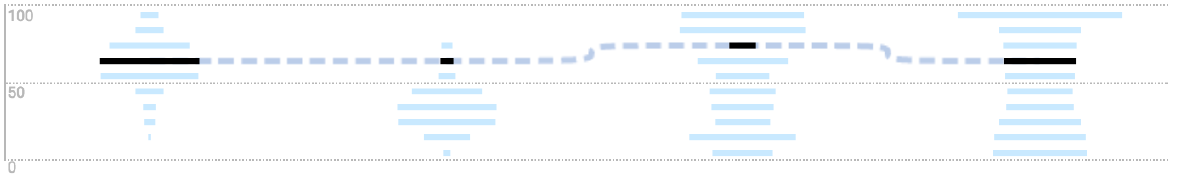
\includegraphics[width=0.8\textwidth]{figures/comp_trend.png}
    \caption{Trajectory of a student and comparison with other students, from \cite{LISSA}}
    \label{fig:comparison_trend}
\end{figure}

So far, all visualizations were concerned with course-level data such as grades or ECTS. However, visualizations can also be used to compare the engagement of students with the course material. Figure \ref{fig:comp_engagement.png} shows a radar plot with different dimensions of interaction. Other than the line for a given student, other thresholds could be shown here. In this example, the average interaction and the student with the highest interaction scores are highlighted. In theory, this could also take some thresholds into account. Some courses have special restrictions on who is allowed to take the final exam, for instance, it might be required to complete 50\% of assignments given out.
More generally, such plots can be used to identify students who are not engaging with the course material enough and thus might be at risk of failing the exam. Figure \ref{fig:comp_engagement.png} also includes recommendations for actions a student could take to increase performance, such as submitting homework on time or retaking a test, in which the student scored lower than usual.

\begin{figure}
    \centering
    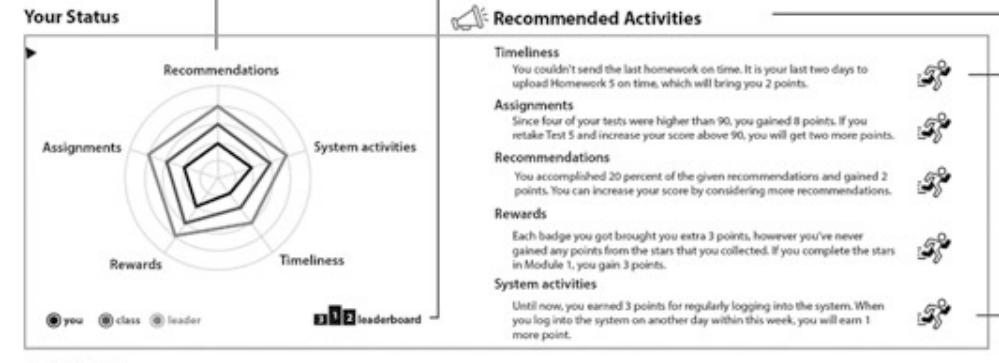
\includegraphics[width=0.8\textwidth]{figures/comp_engagement.png}
    \caption{Radar chart with engagement metrics on the left-hand side, and recommended actions to increase performance on the right, from \cite{StudentFacingDashboard}}
    \label{fig:comp_engagement.png}
\end{figure}

Actual methods for predicting student success are out of scope for this paper, but \cite{DropoutPrediction-SelfRegulatedLearning} shows different predictive models based on the interaction of students with the course material, and suggests good predictive power after about 25\% of the duration of the course, which should leave time for students to adapt their behavior.


One thing to keep in mind when comparing students is choosing the correct comparison group.
For any given course, often there are many students who are enrolled in the online course but do not participate or decide not to take the exam very early on.
Comparing students who actually want to take the exam with those passive students would bias the results. This could lead to a situation where students feel too safe because they are doing more than the average student, but most students doing less are not even planning to take the exam.
Figure \ref{fig:comp_clusters} shows an analysis of different clusters of students, based on their interaction with the course material. This shows that there are distinct groups of students, both with regard to their interaction with course material and their performance, and that interaction with the course material can be used as a predictor of performance, however, the relationship is not necessarily linear.
Such classification should thus be performed before comparing students with each other, to help students make better decisions.

\begin{figure}
    \centering
    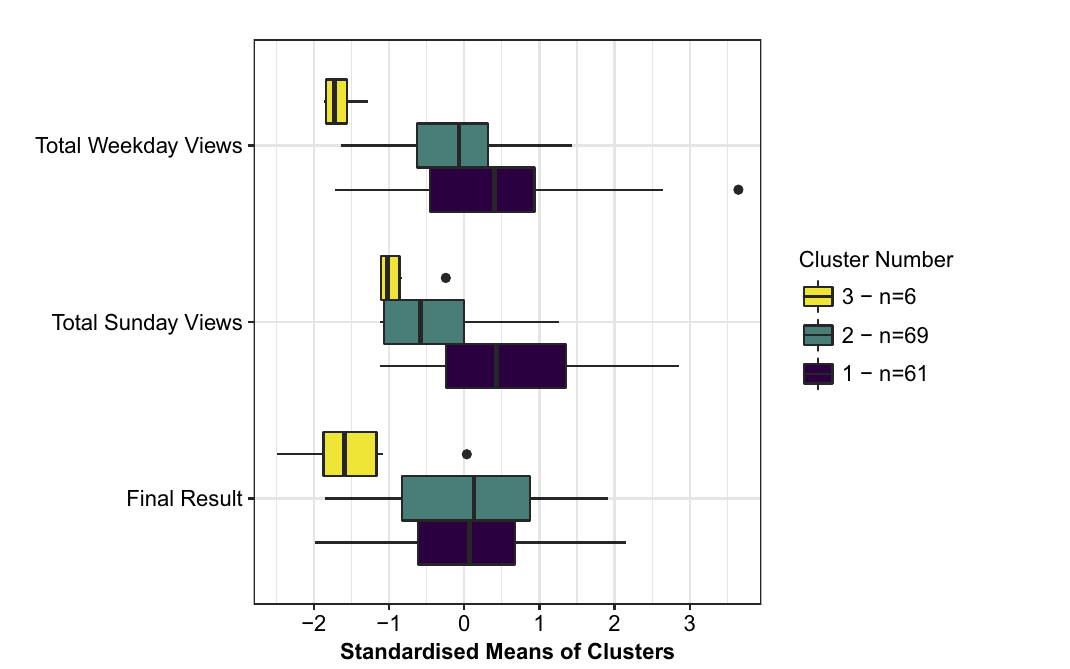
\includegraphics[width=0.8\textwidth]{figures/comp_clusters.png}
    \caption{Clusters of students based on their interaction with the course material, from \cite{PredictionMethods-EarlyWarning}}
    \label{fig:comp_clusters}
\end{figure}

\subsection{Planning}
\label{subsec:planning}

There are multiple phases in a degree program what involve planning. Students might plan their entire degree program upfront, or they might choose which courses to take in the next semester.
Sometimes, students also might have to reconsider if they will be able to pass all exams for the current semester or if they should drop some courses, instead focusing on achieving better grades in fewer courses.

It would be interesting to see, how visualizations could be used to select courses for an upcoming semester, but interesting examples of this are scarce in the literature. Most visualizations do little more than list available courses, with colors to indicate if a course is mandatory or not \cite{Dashboard-StudentProgress}.

Visualizations intended for planning the entire degree program duration might additionally take into account prerequisites for courses. The visualization that comes closest to this is shown in Figure \ref{fig:planning}. Although prerequisites are not explicitly shown, colors indicate which courses are intended for which year of the study program.
Such visualizations can also take into account the number of ECTS credits that need to be achieved in a given semester, an approximated workload for a given course (which in theory should match the ECTS credits, but in practice there usually are quite large differences between courses with the same credits) and the availability of courses. Then, students can plan their degree program in a way that balances their workload while still achieving the necessary credits in a given time frame.

\begin{figure}
    \centering
    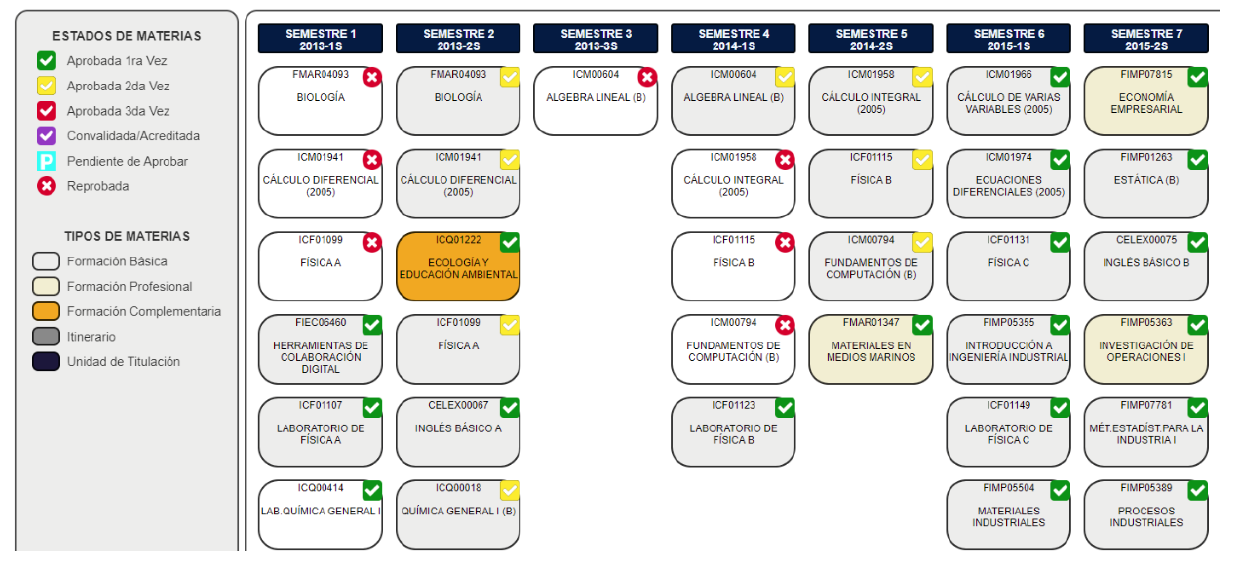
\includegraphics[width=0.8\textwidth]{figures/planning.png}
    \caption{Course selection with indicators showing the year that they are appropriate for, from \cite{LISSA-Planning}}
    \label{fig:planning}
\end{figure}



Figure \ref{fig:planning_2} shows, how such a focus on the credits could look like, with the entire amount of credits that need to be gained (180ECTS for a Bachelor's degree) being displayed as a progress bar up top and multiple sliders for the individual semesters below.
Additionally, visualizations such as in Figure \ref{fig:comparison_exam.png} and \ref{fig:trajectory-finish_1.png} can be useful to inform the planning process.

\begin{figure}
    \begin{minipage}[b]{0.48\textwidth}
        \centering
        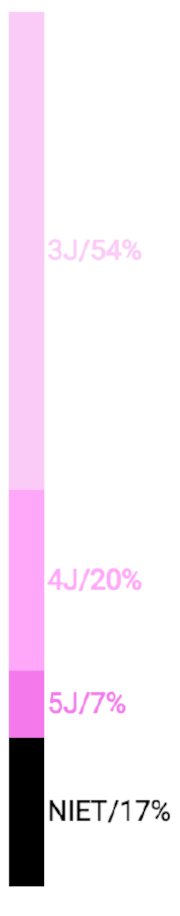
\includegraphics[width=0.3\textwidth]{figures/trajectory-finish_1.png}
        \hfill
        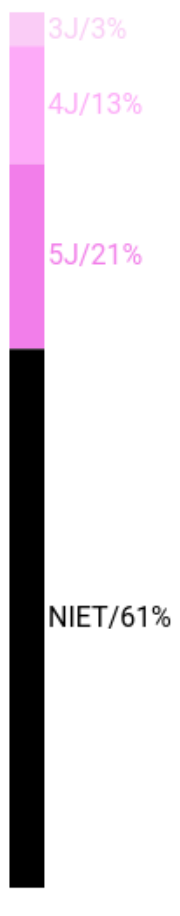
\includegraphics[width=0.3\textwidth]{figures/trajectory-finish_2.png}
        \caption{Estimates for completion of the study program, from \cite{LISSA}}
        \label{fig:trajectory-finish_1.png}
    \end{minipage}
    \hfill
    \begin{minipage}[b]{0.48\textwidth}
        \centering
        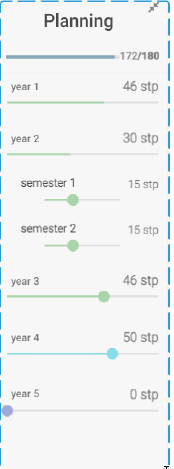
\includegraphics[width=0.8\textwidth]{figures/planning_2.png}
        \caption{Allocation of credits to the semesters, from \cite{LissaLike-StudentSupport}}
        \label{fig:planning_2}
    \end{minipage}
\end{figure}

